% !TEX root = ../Thesis.tex
%
%\documentclass{article}
%\usepackage{graphicx,tikz}
%\usepackage[graphics,tightpage,active]{preview}
%\PreviewEnvironment{tikzpicture}
%\begin{document}
%%%%%%%%%%%%%%%%%%%%%%%%%%%%%%%%%%%%%%%%%%%%%%%%%
	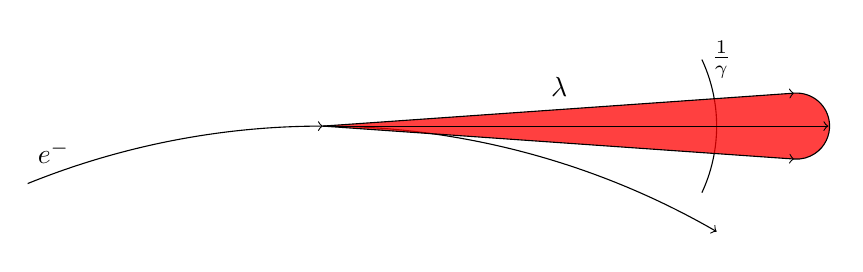
\begin{tikzpicture}
		\clip (-3.75,-1.5) rectangle (6.5,1.25);
		%\draw [help lines] (0,0) grid (5,5);
		% electron arc
			\draw [<-] (0,0) arc (90:110:10) node [above] {$e^-$} arc (110:120:10);
			\draw [->] (0,0) arc (90:60:10);
		% beam angle
			\draw (5,0) arc (0:-25:2);
			\draw (5,0) arc (0:25:2) node [right] {$\frac{1}{\gamma}$};
		% beam
			\def\alpha{4}
			\def\length{6}
			\def\arclength{0.41956087166106248200152636193909} % arclength = tan(\alpha)*\length
			\fill [color=red,nearly opaque] (0,0) -- (\alpha:\length) arc (90+\alpha:-90-\alpha:\arclength) -- cycle; 
			\draw (\alpha:\length) arc (90+\alpha:-90-\alpha:\arclength);
			\node at (3,.5) {$\lambda$};
		% arrows
			\draw [->] (0,0) -- (\alpha:\length);
			\draw [->] (0,0) -- (\length+\arclength,0);
			\draw [->] (0,0) -- (-\alpha:\length);
	\end{tikzpicture}
%%%%%%%%%%%%%%%%%%%%%%%%%%%%%%%%%%%%%%%%%%%%%%%%%
%\end{document}